\section{Machine Condition Monitoring}
% \section{Machine Condition Monitoring And Control}

Machine condition monitoring (MCM) is the process of monitoring the condition of a machine with the intent to predict mechanical wear and failure. Vibration, noise, and temperature measurements are often used as key indicators of the state of the machine. 
Trends in the data provide health information about the machine and help detect machine faults early, which prevents unexpected failure and costly repair \cite{MCMHandbook}. % I would not cite NI here but, if necessary, find a more general reference. NI did not invent MCM ;) \cite{MCM_NI}
%Machine condition monitoring solutions enable predictive maintenance to reduce machine repairs to maximize efficiency.
The need to eliminate catastrophic downtimes due to unexpected breakdowns and unnecessary maintenance costs has made condition monitoring critical for asset utilization and productivity across diverse industries.
The global machine condition monitoring equipment market is expected to grow at a CAGR of 7.6\% between 2015 and 2020 from \$1.5 billion in 2014 to \$2.5 billion by 2020 \cite{ResarchandMarkets15}.

MCM provides vital information about the health of a machine. An organization can use this information to detect warning signs early and avoid unscheduled outages, optimize machine performance, and reduce repair time and maintenance costs. Figure~\ref{fig:MCM_Timeline}  shows a typical machine failure example and the warning signs. The user can detect failure signs months before repair is required, allowing for proper maintenance scheduling and shutdown.

\begin{figure}[ht!]
    \centering
    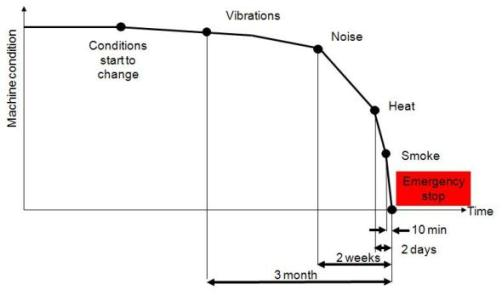
\includegraphics[width=.50\textwidth]{MCM_Timeline}
    \caption{The warning signs of machine failure}
    \label{fig:MCM_Timeline}
\end{figure}

As shown in Figure~\ref{fig:MCM_Timeline}, vibrations are the first warning sign that a machine is prone to failure. This warning sign can provide up to three months of lead time before the actual failure date. Monitoring this data with vibration analysis hardware and software helps predict this failure early and schedule proper maintenance \cite{Randall_VibrationbasedCM}. 

% \subsection{Types of Machine Condition Monitoring}

% Each of the five main varieties of machine condition monitoring serves a different role.
% \begin{itemize}
% \item \emph{Route-based monitoring} involves a technician recording data intermittently with a handheld instrument. This data is then used for trending to determine if more advanced analysis is needed.
% \item \emph{Portable machine diagnostics} is the process of using portable equipment to monitor the health of machinery. Sensors are typically permanently attached to a machine and portable data acquisition equipment is used to read the data.
% \item \emph{Factory assurance test} is used to verify that a finished product meets its design specifications and to determine possible failure modes of the device. 
% \item \emph{Online machine monitoring} is the process of monitoring equipment as it runs. Data is acquired by an embedded device and transmitted to a main server for data analysis and maintenance scheduling. 
% \item \emph{Online machine protection} is the process of actively monitoring equipment as it runs. Data is acquired and analyzed by an embedded device. Limit settings can then be used to control turning on and off machinery.
% \end{itemize}

There are five main types of machine condition monitoring.
\emph{Route-based monitoring} involves a technician recording data intermittently with a handheld instrument. This data is then used to determine if more advanced analysis is needed.
\emph{Portable machine diagnostics} is the process of using portable equipment to monitor the health of machinery. Sensors are typically permanently attached to a machine and portable data acquisition equipment is used to read the data.
\emph{Factory assurance test} is used to verify that a finished product meets its design specifications and to determine possible failure modes of the device. 
\emph{Online machine monitoring} is the process of monitoring equipment as it runs. Data is acquired by an embedded device and transmitted to a main server for data analysis and maintenance scheduling. 
\emph{Online machine protection} is the process of actively monitoring equipment as it runs. Data is acquired and analyzed by an embedded device. Limit settings can then be used to control turning on and off machinery.

% \subsection{Sensors and Signal Processing}

Direct machine condition monitoring is accomplished via sensors, of which the most prevalent types are: accelerometers, tachometers, and proximity probes.  

\begin{itemize}

\item \emph{Accelerometers} are used to monitor vibrations of a machine. These are transducers for measuring the dynamic acceleration of a physical device, and are important to machine monitoring because they monitor system vibrations, which can be used to predict the life cycles of parts and to detect faults in machinery. Among the most common transducers are piezoelectric accelerometers, unbonded strain gage accelerometers, vibrating element accelerometers, and Hall effect accelerometers.

\item \emph{Tachometers} are used to determine the rotational speed of a shaft to provide phase information for the vibration data. These are transducers for measuring the rotational speed of a physical device, and are important to machine monitoring because they provide rotational speed as well as phase information, so that frequency components can be matched to shaft speed and position. Drag torque tachometers are among the most common. 

\item \emph{Proximity Probes} are used to monitor the movement of a shaft. These are transducers for measuring the displacement of a physical device, and are important to machine monitoring because they monitor the movement of a rotating shaft. Proximity probes are usually found in 90-degree offset pairs to map an X-Y plot of the shaft movement. Then imperfections such as misalignment of the shaft, faulty bearings, or other external factors preventing perfect rotation can be prevented. 

\end{itemize}

Most machine condition monitoring sensors require some form of signal conditioning to optimally function, such as excitation power to an accelerometer. Filtering on the signal is also common, to reduce both line noise and unwanted frequency ranges. Once the signals have been acquired, software-based signal processing is used to analyze and display the data from rotating machinery. The analysis can include calculation of overall vibration level (RMS, peak, crest factor); integration from acceleration to velocity or displacement; operation of  online order analysis such as order tracking, order extraction, and order spectra computation; processing of digital and analog tachometer signals; application of limit testing on time data or power spectra; and drawing of a variety of plots ranging from spectral maps to time based plots.

%spectral maps, color maps, waterfall plots, cascade plots, Bode plots, polar plots, orbit plots, time base plots, shaft centerline plots, and Campbell (intensity) plots.

% \subsection{Application Areas}
% Condition monitoring is used in a wide variety of industries. The following is a brief overview of how it works in just a few of them. Certainly condition monitoring can play an important role in any machine with vibrations.

% \subsubsection{Wind Energy}

% To be competitive in the energy market, wind turbines must be operated as cheaply as possible. Maintenance costs for their often remote locations are typically quite high, so route-based monitoring or portable diagnostics systems often don't make sense.  

% Online machine monitoring is often used to monitor wind turbines online from a central location. Technicians can then be deployed to the remote wind farm locations only when maintenance is actually needed.

% Additionally, as companies design larger and more efficient direct-drive turbines, the need for more advanced factory assurance tests becomes increasingly important. Large test cells will need to be built that can monitor turbine designs for up to weeks at a time to verify new multimegawatt designs.

% \subsubsection{Oil and Gas}

% As the cost of reaching oil and gas reserves increases, reducing the operating and maintenance costs of oil and gas assets grows increasingly important. Pumps and drills are often in remote locations where technician expenses are high.

% Using online condition monitoring techniques, you can monitor pumps, wells, and refineries from a central location and only deploy maintenance personnel when necessary, saving operating and maintenance costs.

% The oil and gas industry is also increasingly under pressure for improved safety and oversight. Condition monitoring offers the opportunity to discover possible defects weeks before a technician may find them, and it provides advantages over performing maintenance at only manufacturer-recommended intervals, which may not be early enough to prevent a catastrophic failure.





